\chapter{Theory}
\label{chapter:theory}

\section{Machine Learning}
Machine learning is a branch of computer science that deals with building and analyzing systems that are able to learn from data. Algorithms based on such analysis involve constructing a model from a given dataset, and then using this model to perform required tasks. Machine learning techniques can broadly be divided into two categories - supervised learning, and unsupervised learning.

\begin{itemize}
    \item{\textbf{Supervised Learning} Methods falling in this category operate in two phases. In the first step, the availability of training data is assumed, which is used to build a model so that it takes into account the structure of the given dataset. In the second step, this model is used to make predictions on the testing data (the real world data). This is the data that the model has not seen yet, and is required to make predictions on.}
    \item{\textbf{Unsupervised Learning} Methods falling under this category operate in a single phase. It starts with a model with zero knowledge about the structure of the given dataset. As data is fed into the model, it continuously learns the structure of the given dataset and calculates the predictions based on this knowledge. The main difference between this family of algorithms and supervised learning algorithms is the presence/absence of training labels.}
\end{itemize}

The primary focus in this thesis remains on supervised learning methods.\\

\section{Classification Methods}
Text classification is a subset of machine learning algorithms used to assign specific categories to pieces of data. It is one of the msot fundamental problems in machine learning. More precisely, given some sample information (such as what kind of data points are to be assigned to which category), these algorithms allow for assigning categories to unseen data points. Under the scope of this thesis, the data is always assumed to be English-text. Since machine learning algorithms only deal with real numbers, a necessary first step is the conversion of natural language text into real numbers. The work presented in this thesis makes extensive use of supervised text classification algorithms.\\

Given a dataset $\mathbf{X}$, it is required to separate the samples contained within the dataset into two (or more than two, depending on the input) classes. Formally, given a dataset that contains $N$ instances,

\begin{center}
    $\{(x_n, y_n)\}_{n = 1}^{N}$,
\end{center}

where each instance ($x_n, y_n$) is of the form,

\begin{center}
    $[(x_{n, 1}, x_{n, 2}, ... x_{n, D}), y_{n}]$,
\end{center}

each $x_{n, d}$ being the value of the feature $d \in [1, D]$, and $y_n$ being the label of the sample which can take a limited number of possible values, the aim is to calculate the value of $y_n$ given this feature information. In the supervised learning problem, this dataset is divided into two parts - training data (which contains the $y_n$ values for each instance), and test data (no information on $y_n$ is available), and the problem is to identify the values of $y_n$ in the test data given only the information present in the training data. On the other hand, in unsupervised text classification, the model is required to identify the $y_n$ values given only the values for $x_n$, there being no distinction between training and test data.\\

The performance of a particular classifier varies with the type of the data to be classified. Not all classifiers are good for all classes of problems. Some classifiers suit a particular problem more than some others; choosing a classifier for a problem still remains a decision which may or may not be completely scientific, even though a lot of work has been done to correlate classifier performance with data type.

\section{Support Vector Machines}
Support Vector Machines (SVMs) form a fairly popular class of machine learning algorithms used mainly for binary classification and regression analysis. Given the training data, the goal of an SVM is to find a decision boundary (a hyperplane in a high or infinite dimensional space) that separates the two classes of data while maximizing the distance of the boundary from any data point. The resulting decision function is fully specified by a (usually small) subset of the data, and the points in this subset are referred to as support vectors.\\

Most classifiers resort to a distance function, in some form or the other, that can provide a similarity measurement between two points. In the simplest form of an SVM, the distance function is simply the dot product between two points, and such SVMs are referred to as \emph{Linear Support Vector Machines}. In the case that a simple linear SVM is not able to find a sufficiently accurate decision boundary that can separate the data points into two classes (simply because the input data is not linearly separable), the so-called \emph{kernel trick} is used, which involves transforming the data from a low dimensional space to a much higher dimensional feature space (in which the input data may be separable) using an appropriate function

\begin{center}
    $\phi(x): \mathbb{R}^{L} \rightarrow \mathbb{R}^H (L \ll H)$
\end{center}

and then using the kernel function $k(\phi(x), \phi(y))$ to actually perform the separation. The trick involved is that even though the transformation $\phi(x)$ may be expensive, computing the final similarity value $k(\phi(x), \phi(y))$ is not.\\

Some of the most popular kernel functions include
\begin{itemize}
    \item{Linear (the simple SVM) - $k(x, y) = (x \cdot y)$ }
    \item{Polynomial - $k(x, y) = (\gamma x \cdot y + c)^{d}$}
    \item{Radial Basis - $k(x, y) = \exp(-\gamma {| x - y |}^{2})$}
    \item{Sigmoid - $k(x, y) = \tanh(\gamma x \cdot y + c)$}
\end{itemize}

Figure~\ref{fig:svm_linear_classify} shows a scenario where a support vector machine is used to classify two sets of points that are generated from partially overlapping Gaussian distributions. This dataset can be classified by a linear kernel SVM since this data is linearly separable.\\

\begin{figure}[t!]
    \centering
    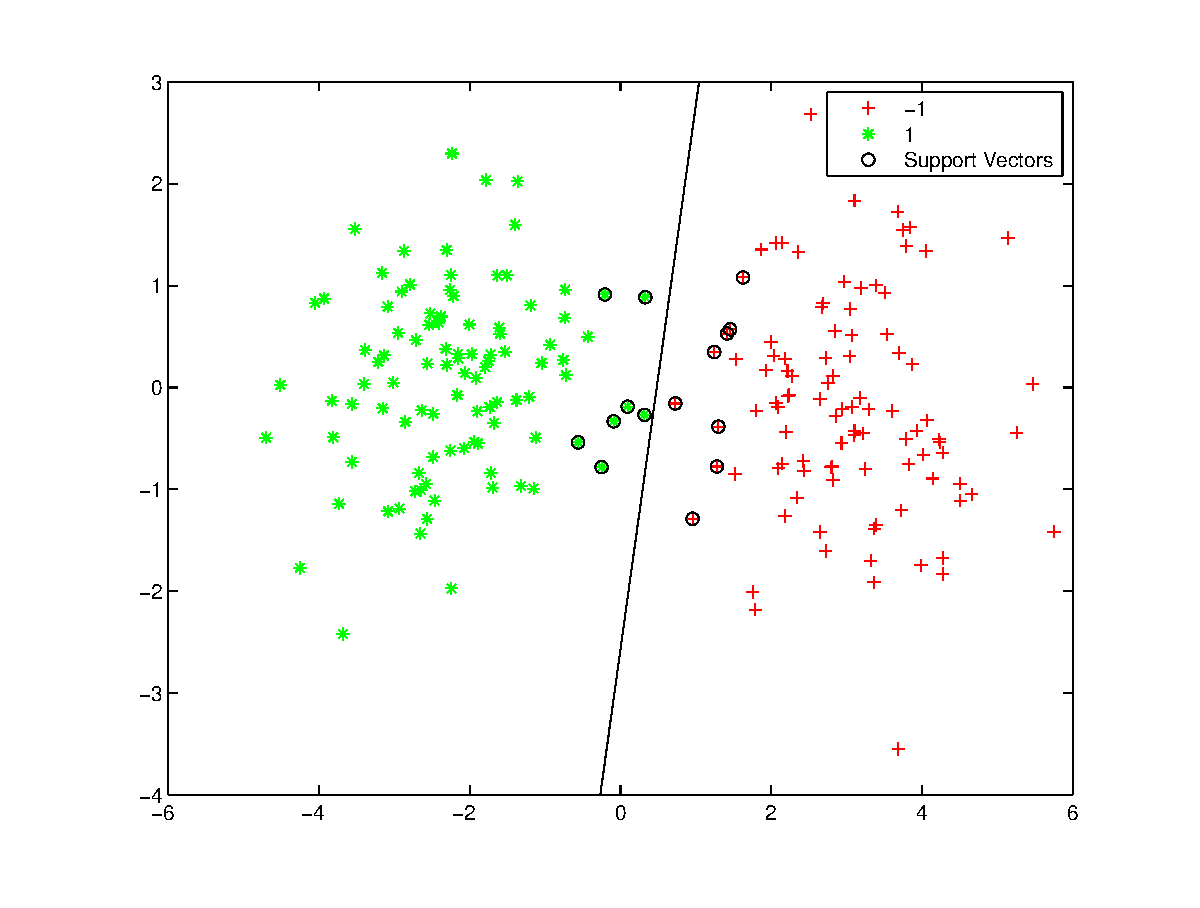
\includegraphics[width=0.8\textwidth]{svm_linear_classification.eps}
    \caption{Classification using a linear kernel SVM}
    \label{fig:svm_linear_classify}
\end{figure}

However, for a case when the data is not linearly separable and looks like as shown in Figure~\ref{fig:svm_non_linear_data}, the linear kernel performs poorly. This is shown in Figure~\ref{fig:svm_non_linear_classify_linear}. When the dataset has such characteristics, a much better option is to use a kernel that is able to work with such data. For instance, an RBF kernel draws a much better boundary in this case, as shown in Figure~\ref{fig:svm_non_linear_classify_rbf}.\\

\begin{figure}[t!]
    \centering
    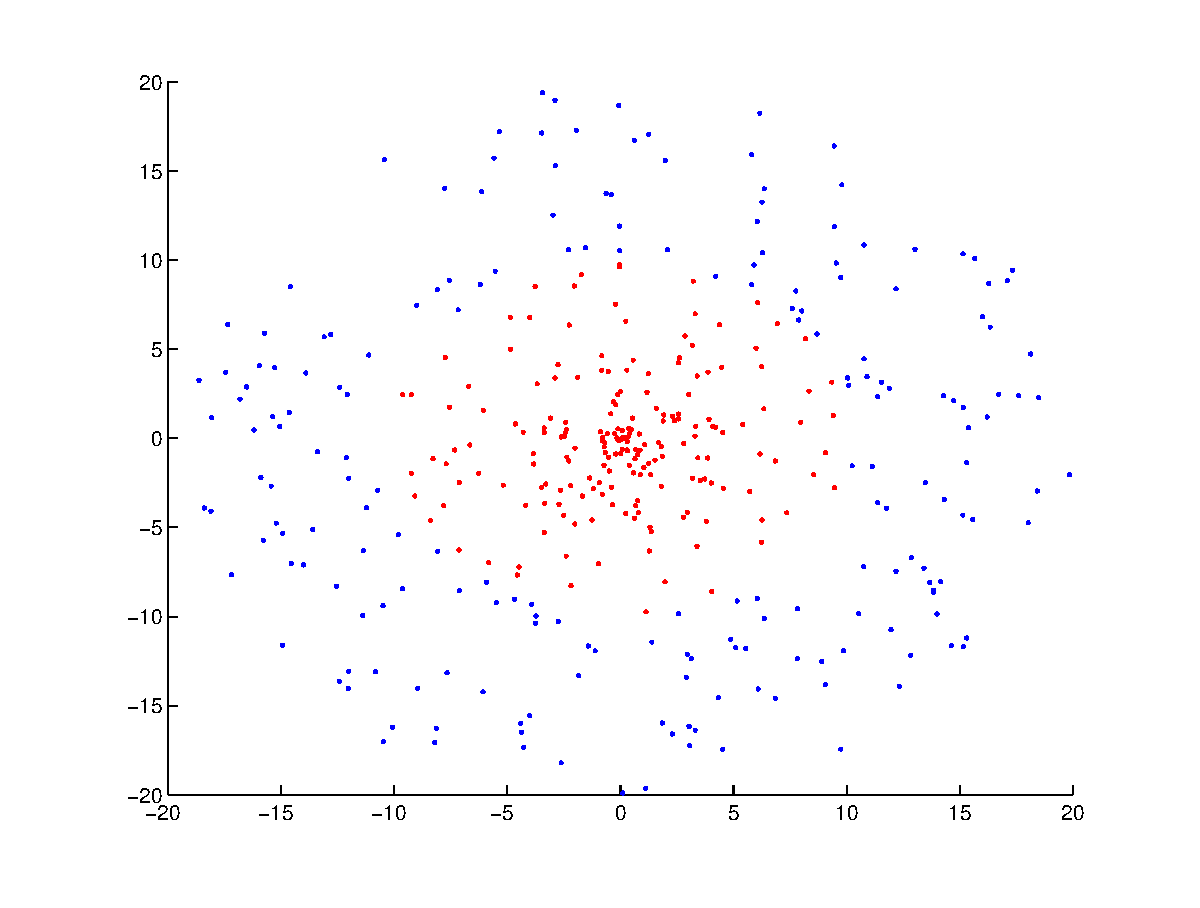
\includegraphics[width=0.8\textwidth]{svm_non_linear_data.eps}
    \caption{A dataset which is not linearly separable}
    \label{fig:svm_non_linear_data}
\end{figure}

\begin{figure}[t!]
    \centering
    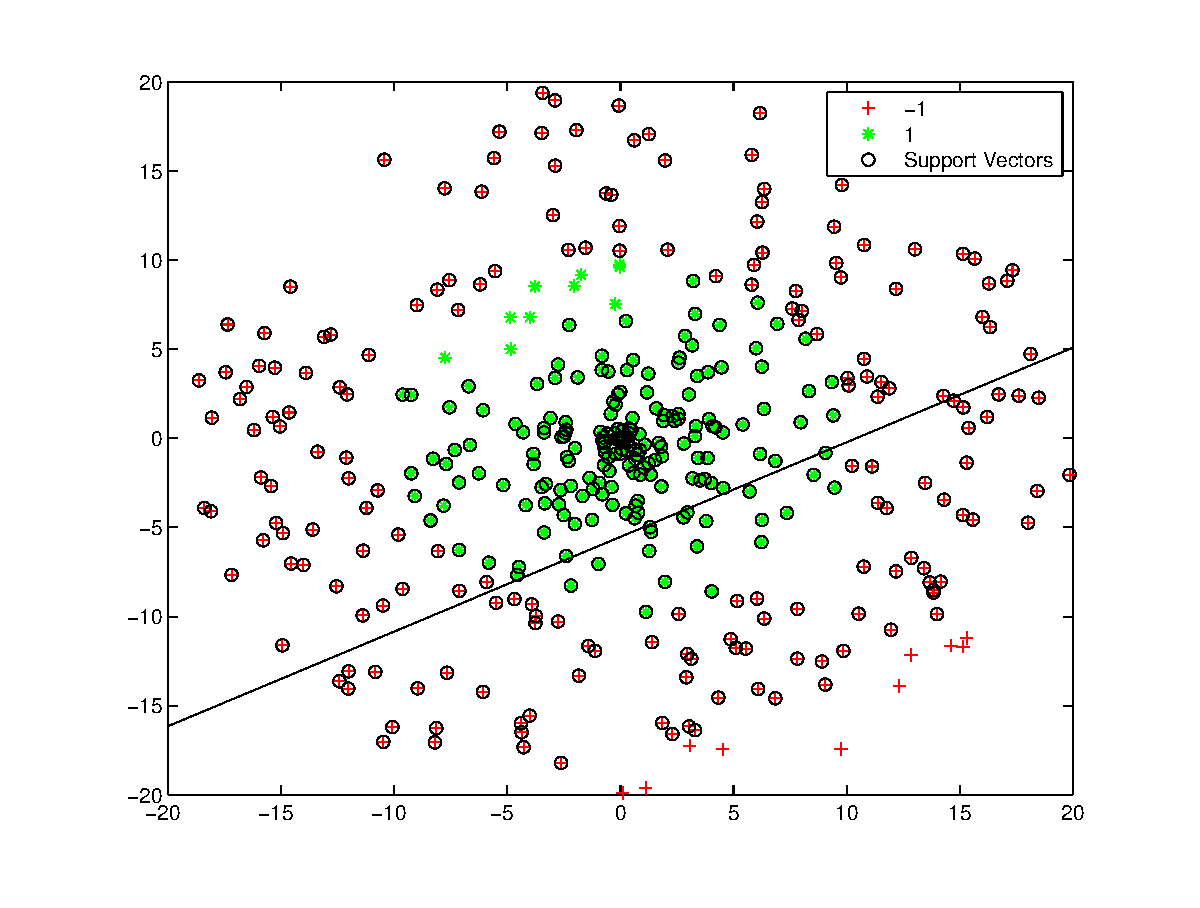
\includegraphics[width=0.8\textwidth]{svm_non_linear_classify_linear.eps}
    \caption{Dataset for Figure~\ref{fig:svm_non_linear_data} being classified using a linear kernel}
    \label{fig:svm_non_linear_classify_linear}
\end{figure}

\begin{figure}[t!]
    \centering
    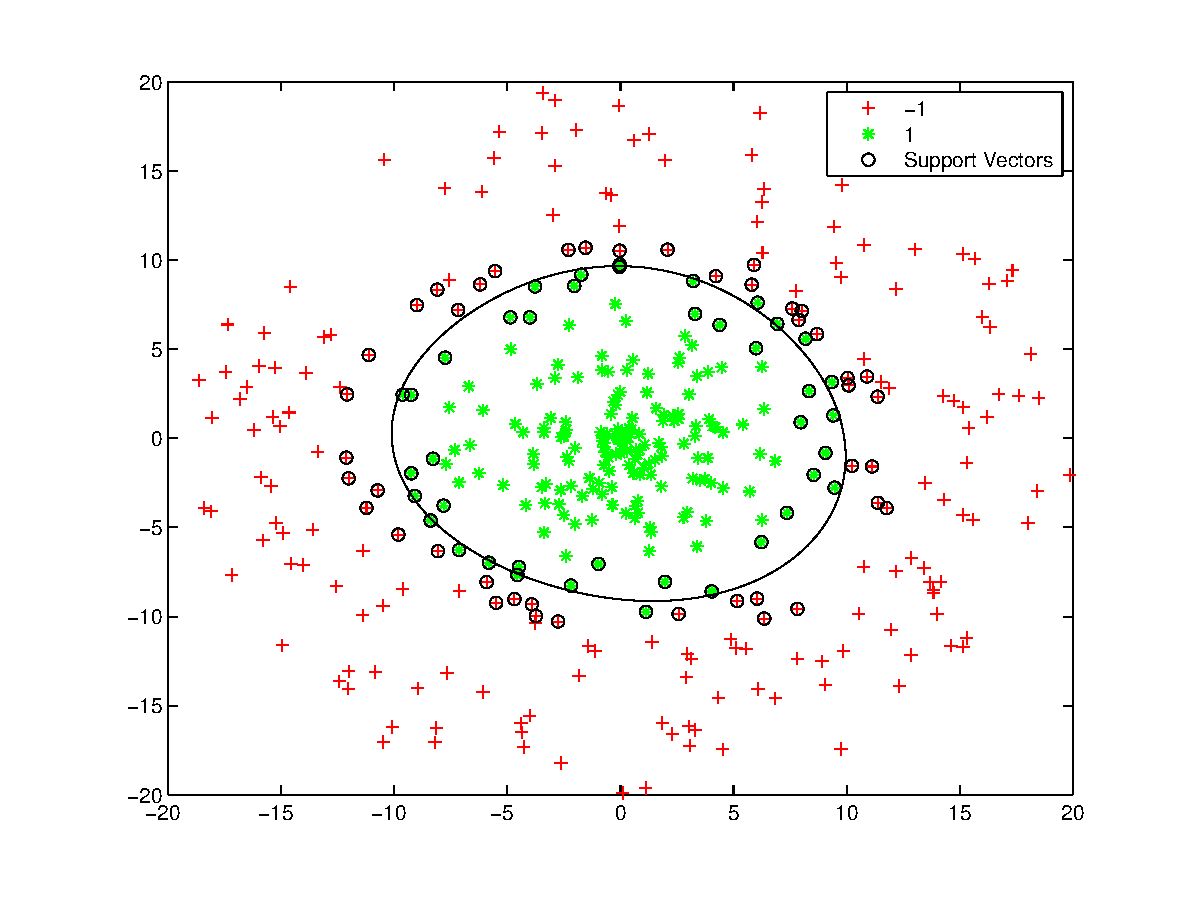
\includegraphics[width=0.8\textwidth]{svm_non_linear_classify_rbf.eps}
    \caption{Dataset for Figure~\ref{fig:svm_non_linear_data} being classified using an RBF kernel}
    \label{fig:svm_non_linear_classify_rbf}
\end{figure}

Intuitively, the work done by the $\phi(x)$ function can be visualized from Figure~\ref{fig:svm_non_linear_data}, and Figure~\ref{fig:svm_non_linear_data_3d}. Figure~\ref{fig:svm_non_linear_data} shows the original dataset that the linear kernel failed to classify with reasonable accuracy. A simple transformation can be applied in this case to make the data separable, transforming the two dimensional input to a three dimensional input by adding the following transformation.\\

\begin{center}
    $ \phi(x) = \sqrt{x_1^2 + x_2^2} $
\end{center}

This transformation transforms the input data in the shape of a three dimensional cone which is separated into two parts by a simple plane in three dimensions. The points in the inner circle form the tip and the surrounding areas of the cone, while the rest of the cone is constituted by the remaining points. The resulting data looks like Figure~\ref{fig:svm_non_linear_data_3d}.\\

\begin{figure}[t!]
    \centering
    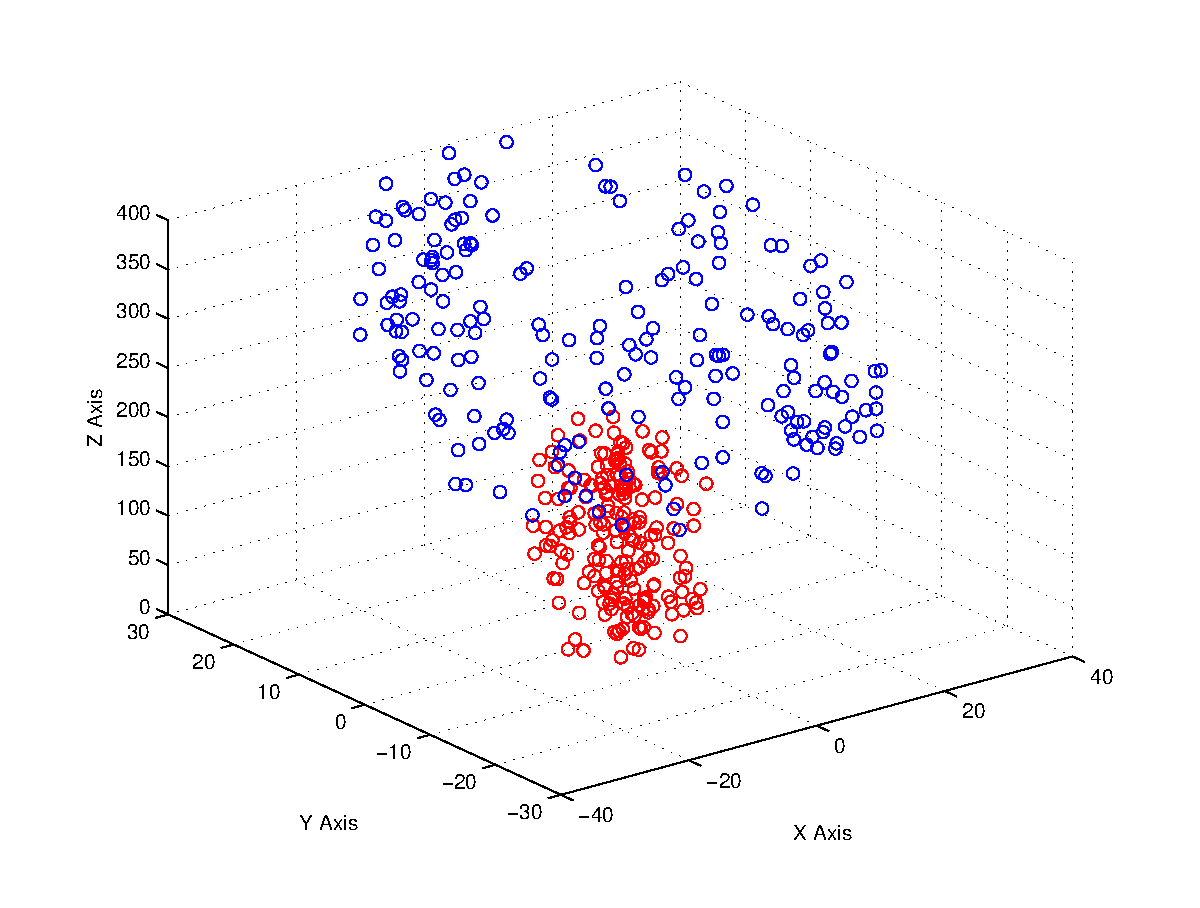
\includegraphics[width=0.8\textwidth]{svm_non_linear_data_3d.eps}
    \caption{The dataset from Figure~\ref{fig:svm_non_linear_data}, exported into a three dimensional space, which can now be separated by a linear plane}
    \label{fig:svm_non_linear_data_3d}
\end{figure}

The code for this transformation (including the generation of the original data) is shown in Listing~\ref{lst:svm_linear_classify}.\\

\lstinputlisting[language=Matlab,caption={Generating the dataset to be classified by a linear classifier},label={lst:svm_linear_classify}]{code/svm_linear_classify.m}

\section{Text Representation}
Machine learning algorithms are designed to operate on real values. To classify documents, a prerequisite is to convert the natural language text to a format that such an algorithm can understand and work on. One such format is the vector space model. Processes to convert natural language text to such formats include obtaining text from documents, building a vocabulary, text preprocessing (such as tokenization, stemming, and stop words removal), and converting terms to actual usable feature values. The processes may differ slightly for different languages. For instance, tokenization for English text is different from tokenization for Chinese text because of differences in word boundaries. But these differences are minor and do not change the overall flow.

\subsection{Preprocessing}
Preprocessing documents typically involves all the steps that are needed to be performed before proceeding on to extracting meaningful information from text that the classifier could handle. Text documents in their original forms normally contain a lot of redundant information that usually does not affect how a classifier behaves. Preprocessing removes all the noise, and brings a document in a state where it can be used for scoring. The following are the various filters that are applied.

\begin{itemize}
    \item{
    Extraction - Data extraction involves extracting relevant data out of documents. Often, documents are unstructured, poorly structured, or are in a format such as XML or HTML. In such cases, the documents in their original forms contain a lot of redundant information. Extracting relevant data by using methods like parsing brings documents to a state where they are ready to be tokenized.
    }
    \item{
    Tokenization - Tokenization is the process of splitting a sequence of words into distinct pieces of alphanumeric characters, called tokens. Extra characters which are not needed, such as punctuations and white spaces and linebreaks are removed. For instance, tokenizing the text \emph{"The quick, brown, fox jumps over the lazy dog;"} results in the following list of tokens - \\
    \begin{center}
        \begin{verbatim} the | quick | brown | fox | jumps | over | the | lazy | dog \end{verbatim}
    \end{center}
    In most cases, tokens are split using whitespcaces, line breaks, or punctuation characters. Splitting on white spaces may also result in some loss of information. For instance, if the string \emph{San Francisco} appears in the text, then the tokens extracted will be \emph{San} and \emph{Francisco}, whereas the correct tokenization should treat both the terms in one token. One approach to solving such problems is using n-grams, which is explained later in this section.
    }
    \item{
    Stop Words Removal - Some of the words in the English language such as \emph{and}, \emph{the}, and \emph{a}, besides some others appear in almost every text. These words add very little meaning to the text on the whole, and their frequency of occurrence is very high. Consequently, since these words appear a lot in almost every document, it may lead to high and inaccurate similarity scores between two documents; the best option is to remove such words from the text.
    }
    \item{
    Stemming - Stemming is the process of reducing words to their root form, usually by stripping some characters from the word endings. A strict requirement for stemming is that related words must stem to the same final word. For instance, the words \emph{car}, \emph{cars}, \emph{car's} and \emph{car`s}, must all stem to the same word \emph{car}. This helps in removing unnecessary information from the text which would otherwise inflate the vocabulary with low-signal information.
    }
\end{itemize}

\subsection{Representation and Vector Space Classification}
After a document has been preprocessed, it needs to be represented in terms of the useful content that it has, such that the relative importance of each word has been taken into account. Since a preprocessed document is just a collection of tokens, it can be represented as a vector

$$x_n = (x_{n, 1}, x_{n, 2}, ... , x_{n, D})$$

where each dimension $x_{n, d}$ corresponds to a token, and the value depends on its occurrence, either only in the document, or in the document as well as in the entire corpus. This approach is called the bag-of-words model. For instance, consider two simple HTML documents containing English text,

\begin{center}
    \begin{verbatim}
    <html>
        <head> <title>Munich</title> </head>
        <body> We are headquartered in Munich, Germany. </body>
    </html>
    \end{verbatim}
    and
    \begin{verbatim}
    <html>
        <head> <title>Berlin</title> </head>
        <body> We also have an office in Berlin, Germany. </body>
    </html>
    \end{verbatim}
\end{center}

After data extraction, the documents look like the following,

\begin{center}
    \begin{verbatim} Munich We are headquartered in Munich, Germany \end{verbatim}
    and
    \begin{verbatim} Berlin We also have an office in Berlin, Germany \end{verbatim}
\end{center}

It can be seen that all the HTML tags have been stripped off and only the relevant information remains. The documents are further subjected to token extraction, after which they look like the following,

\begin{center}
    \begin{verbatim} Munich | We | are | headquartered | in | Munich | Germany \end{verbatim}
    and
    \begin{verbatim} Berlin | We | also | have | an | office | in | Berlin | Germany \end{verbatim}
\end{center}

The next step in preprocessing involves removing stop words and stemming. After removing the stop words, the only tokens that are left in the corpus include ``Munich'', ``headquartered'', ``office'', and ``Germany'', forming a term dictionary over which will not really illustrate the vector space representation in a good way. Hence, ignoring the stop words removal for the sake of this example, the corpus looks like the following after stemming

\begin{center}
    \begin{verbatim}
        {
            'We': 1,
            'are': 2,
            'headquarter': 3,
            'in': 4,
            'Munich': 5,
            'Germany': 6,
            'also': 6,
            'have': 8,
            'an': 9,
            'office': 10,
            'Berlin': 11
        }
    \end{verbatim}
\end{center}

and the documents are then represented as the following vectors

\begin{center}
    \begin{verbatim}
                {1, 1, 1, 1, 2, 1, 0, 0, 0, 0, 0}
    \end{verbatim}
    and
    \begin{verbatim}
                {1, 0, 0, 1, 0, 1, 1, 1, 1, 1, 2}
    \end{verbatim}
\end{center}

where each value represents the number of times the particular token appeared in the corresponding document. The order of words does not matter; the features simply indicate whether or not the word appeared in the document.

In this example, the values represent term frequencies. A slight improvement is to divide the term weights with the total number of terms in the document, which assigns the feature values while also taking into account the relative importance of the term in the document. An even better improvement is to use the $\mathrm{tf-idf}$ value, which (for a term in the document) is defined as

$$\mathbf{tfidf}_{t, d} = \mathbf{tf}_{t, d} * \mathbf{idf}_{t}$$

where $\mathrm{tf}_{t, d}$ is the term frequency of the term $\mathbf{t}$ in document $\mathbf{d}$, and $\mathrm{idf}_{t}$ is the inverse document frequency of the term $\mathbf{t}$ across the entire collection of documents, usually defined as $\log(N / \mathrm{df_{t}})$, where $\mathrm{N}$ is the total number of documents, and $df_{t}$ is the number of times this term appears in the entire collection of documents. The main idea here is to reduce the term frequency weight of a term by a factor that increases proportional to its frequency in the corpus. This tf-idf value is the highest when the term occurs many times within a small number of documents, and the lowest when the term occurs in almost all documents. Hence it provides a good representation of a document in the vector space format. This representation can now be used to calculate the similarity between two documents. The standard way for this is to compute the dot product between the two vector representations

$$\mathbf{sim(x, y)} = \frac{\vec{\mathbf{x}} \cdot \vec{\mathbf{y}}}{|\vec{\mathbf{x}}| | \vec{\mathbf{y}}|}$$

\section{Ensemble Learning}
Ensemble Learning is a class of supervised learning algorithms that use multiple models instead of a single one to obtain better predictions. A common problem with classifiers is that not all classifiers are suited for all kinds of problems. Ensembles of classifiers involve combinining multiple classifiers to construct an expectantly better classifier. The performance of an ensemble is not guaranteed to be better than the individual classifiers, but depending on the problem, an ensemble usually outperforms its constituent classifiers by a fair margin. But like almost all machine learning methods, a generalization cannot be made and it depends a lot on the problem at hand. Using ensemble learning requires performing more computation, but yields better results when the classifiers are not similar to each other.

\subsection{Bagging}
Bagging, also referred to as Bootstrap Aggregation, is one of the most basic forms of ensemble learning. Given a training dataset $D$ containing $N$ samples, each sample having $D$ different features, the aim of bagging is to combine $M$ classifiers, each trained using a different subset of the main data, such that every classifier learns about a different structure of the input data. When the outputs from all the constituent classifiers are combined, the final output is expected to be better than the individual predictions. Bagging requires that the entire system should not be stable, so that when the training data changes by even small amounts, the resulting classifiers are different \cite{quinlan1996bagging}. A consequence of this was also presented in \cite{breiman1996bagging}, where it was noted that for unstable classifiers, bagging introduces improvements in the net classifier accuracy. On the other hand, if the underlying classifiers are already strong and stable, the performance may degrade a little \cite{breiman1996bagging}. Bagging is often known as the less risky approach, in that there is a high chance that using bagging improves the performance of the classifier.\\

To train different classifiers on a different subset of the data, the training data is either split on the number of samples, or on the number of features. In the first case, $N' (< N)$ samples are picked with replacement, and each time a new classifier is trained using the new dataset. Since the data points are picked with replacement, some of the data points may be common to some classifiers. In the second case, every new classifier is trained using $M' (< M)$ features with replacement. Whenever the ensemble is required to make a prediction on a new sample, a majority vote from all the constituent classifiers is taken, which becomes the final output of the ensemble.

\subsection{Boosting}
The original hypothesis behind Boosting was the notion that a set of weak learners can be trained to form a strong learner \cite{kearns1988thoughts}. Boosting aims to build an ensemble of classifiers by iteratively training weak classifiers on a distribution, and then finally putting them all together to build a strong classifier. In the training phase, the classifiers are trained one by one. Each training instance is assigned a numeric weight, which is the same for all samples in the beginning. After the first classifier has been trained, the weights for the points which were misclassified are increased, and the resulting input data (along with the modified weight values) is fed to the second classifier. This process continues until the last classifier has been trained. This way, each classifier has an incentive to focus more on classifying correctly those points which the previous classifier classified incorrectly.\\

Each classifier's performance is maintained in a vector (usually named $\alpha$). Whenever a new point has to be classified, the individual predictions are obtained from the constituent classifiers, and a weighted sum (from the $\alpha$ values) is taken across all the classifiers to obtain the final prediction. One of the very popular Boosting techniques is Adaptive Boosting, originally presented in \cite{freund1995desicion}. The main aim of Boosting is to build a strong classifier from a set of weak classifiers. To that effect, even classifiers only slightly better than random are considered useful, because in the final predictions, they will still contribute positively to the aggregate prediction by behaving like their inverses because of having negative coefficients in the final linear combination of classifiers.\\

The algorithm used to train a model over a dataset is the following.

\begin{enumerate}
    \item{Initialize the sample weights $w_n = 1/N$, for $n = 1, 2, ..., N$}
    \item{
    For $m = 1, 2, ..., M$:
    \begin{itemize}
        \item{Train a classifier $\mathbf{y_m(x)}$ on the training data using the sample weights $\mathbf{w}$}
        \item{Calculate $$\epsilon_m = \frac{\displaystyle \sum_{n = 1}^{N} w_n I_n}{\displaystyle \sum_{n = 1}^{N} w_n}$$ where $I(y_m(x_n) \neq y_n)$ is the indicator function and equals 1 when the predicted label $y_m(x_n) \neq$ the actual label $y_n$, and 0 otherwise}
        \item{Set $$\alpha_m = \log(\frac{1 - \epsilon_m}{\epsilon_m})$$}
        \item{Update $\mathbf{w}$ using $$w_n := w_n \exp(\alpha_m I(y_m(x_n) \neq y_n))$$}
    \end{itemize}
    }
\end{enumerate}

After all the models have been trained, the prediction for an instance $x_n$ is obtained by calculating $$sign(\displaystyle \sum_{m = 1}^{M} \alpha_m y_m(x_n))$$

\subsection{Stacking}
Stacking, also called Stacked Generalization was first introduced in \cite{wolpert1992stacked}, and obtains predictions by a two step process. It is assumed that there exists a training input matrix that has $N$ rows for $D$ samples, and $D$ columns for $D$ features. In the first step, $M$ distinct classifiers are trained on the training data. After the classifiers have been trained, a new dataset of $N$ rows and $M$ columns is generated, each column being populated by predictions for each of the $M$ classifiers. This new dataset forms the training data for a second level classifier, from which the final prediction is obtained. The process for prediction from a Stacking ensemble follows a similar path. Given a sample $x_n$ of the form $[(x_{n, 1}, x_{n, 2}, ... x_{n, D})]$, it is first run through the $M$ classifiers to obtain $M$ predictions $(y_m)$ for $m = 1, 2, ..., M$. These values are then fed to the second level classifier, which yields the final label.\\

\begin{figure}
    \centering
    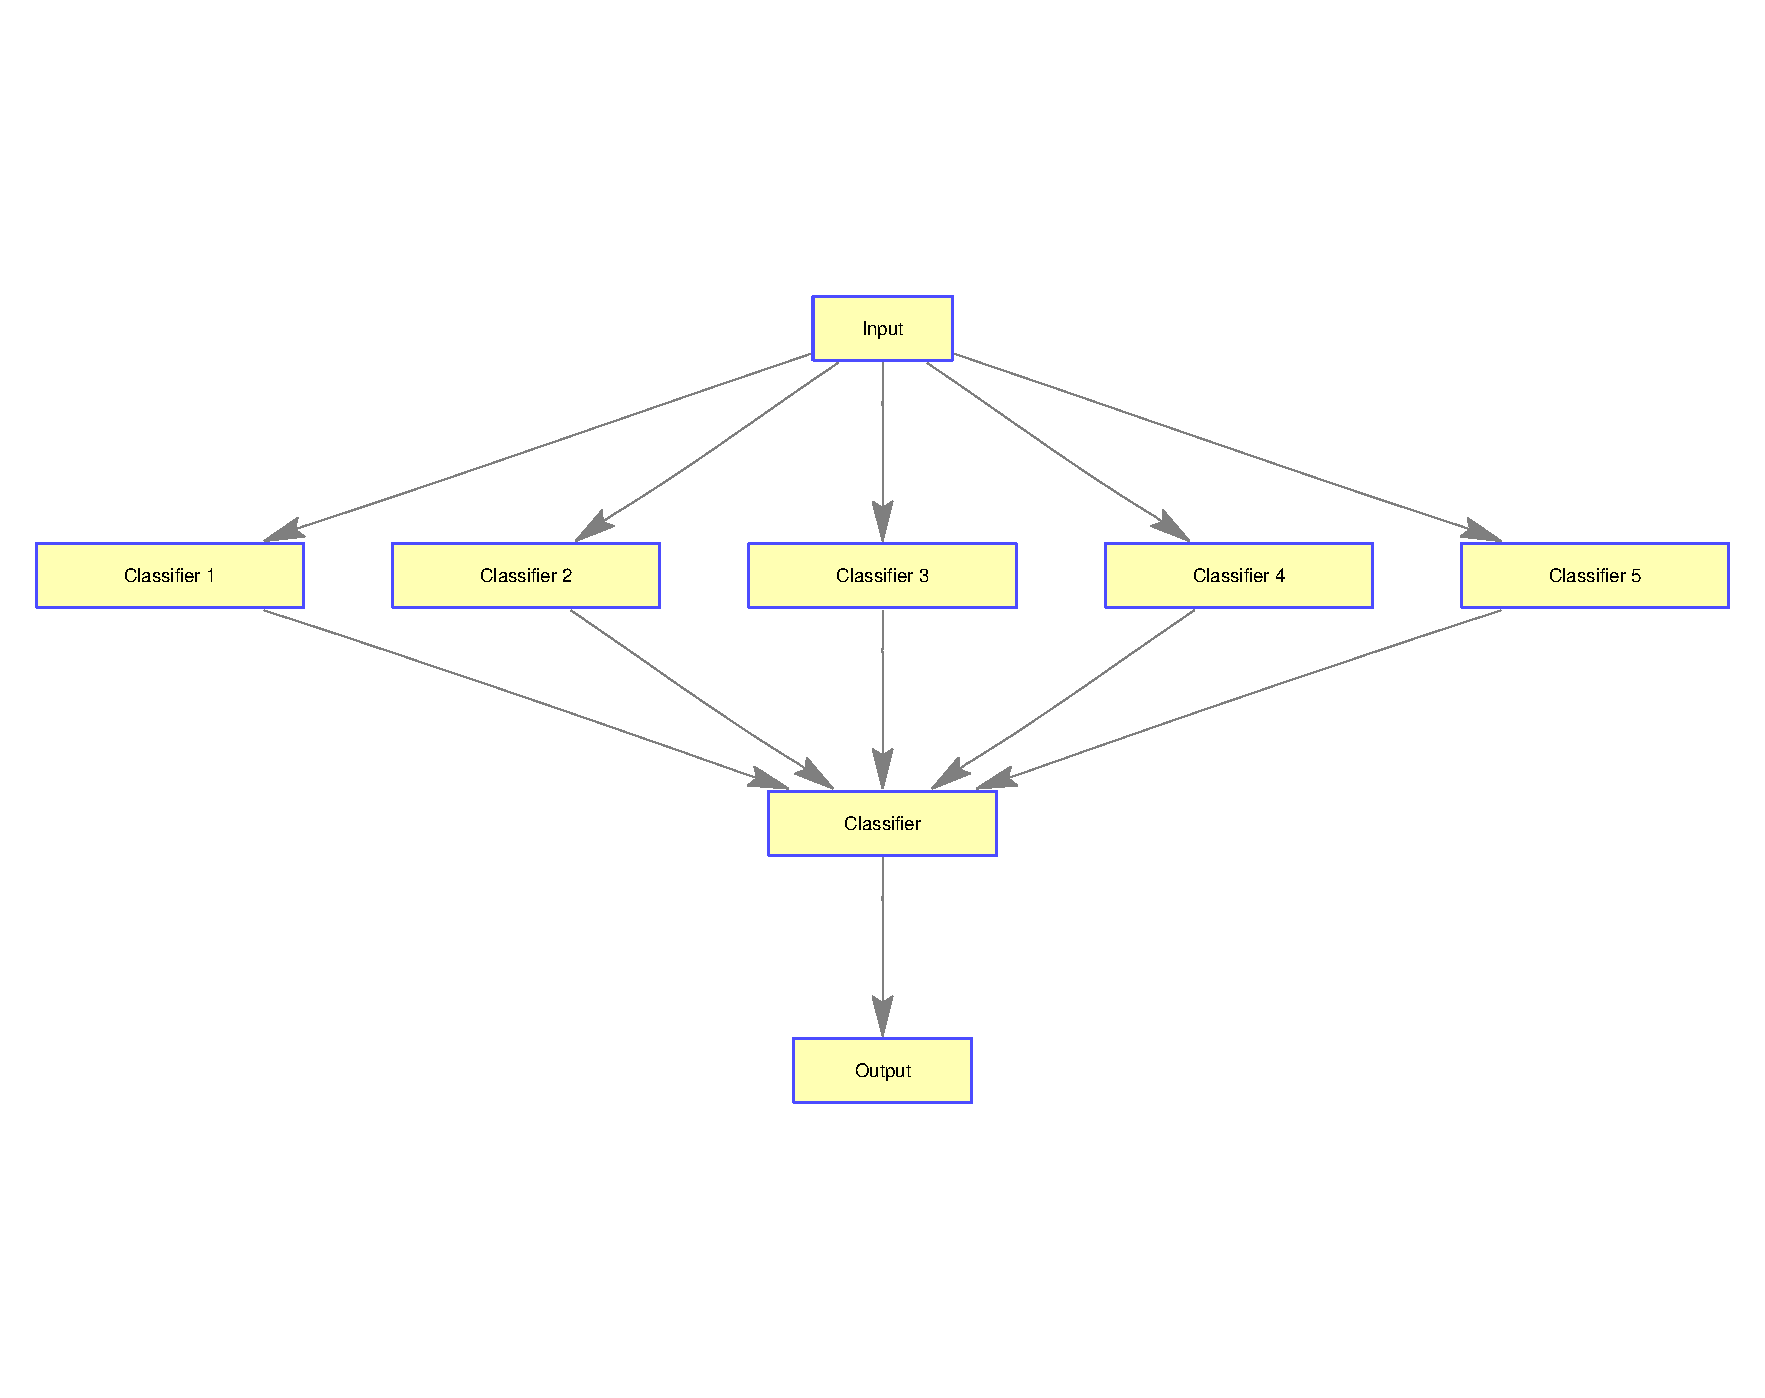
\includegraphics[width=0.8\textwidth]{stacking_flow.eps}
    \caption{Stacking}
    \label{fig:stacking_flow}
\end{figure}

Figure~\ref{fig:stacking_flow} illustrates how stacking works when there are 5 classifiers at the first level. The node ``Input'' refers to the sample $x_n$ for which the prediction is to be made. It is fed to each classifier, and the resulting predictions from the classifiers form an $M$ dimensional vector, which is then fed to the main classifier at the second level, which then gives the final label. Two of the most common schemes for training classifiers at the first level include bootstrapping (training different classifiers using different subsets of data) and feature sampling (using different features as inputs for different classifiers). Stacking is one of the best ensemble learning methods that has proven to be successful in a number of works, as well as in the real world. The study done in \cite{dvzeroski2004combining} experimented with a number of datasets to compare stacking against multiple schemes for combining classifiers, to discover that a stacking ensemble performs much better than when classifiers are combined using the \emph{voting} or \emph{select-best} schemes. The nature of inputs for the second level classifier were studied in \cite{ting2011issues}. This work concluded that much better results can be obtained if the confidence values from the first level classifiers are included in the input for the higher level model. Stacking was also employed by the winning team at the Netflix prize \cite{koren2009bellkor}, in which the solution included meta features as inputs (number of users and number of movie ratings) in addition to using the normal feature vectors.
